\documentclass{homework}

\usepackage[a4paper,margin=1in]{geometry}
\usepackage{kotex}
\usepackage{environ}

\usepackage{amsmath}
\usepackage{amssymb}
\usepackage{braket}

\usepackage{graphicx}

\usepackage{tikz}
\usetikzlibrary{arrows,shapes.gates.logic.US,shapes.gates.logic.IEC,calc}

\usepackage{xparse}
\usepackage{xcolor}

\NewEnviron{twocolumnproof}{
    \newcommand{\justification}[1]{ & {\quad} & \text{##1}}
    \begin{align*}
    & \text{Steps} \justification{Justifications} \\
    \hline \\[-2ex]
    \BODY
    \end{align*}
    }

\newcommand{\hwname}{이주헌}
\newcommand{\hwemail}{20191629}
\newcommand{\hwnum}{1}

\newcommand{\hwtype}{Homework}
\newcommand{\hwclass}{CSE3015}

\begin{document}

\maketitle

\question*{What is different between synchronous sequential systems and asynchronous sequential systems? Give examples how the circuits operate.}

Sequential systems are dependent not only on current set of inputs, but also on previous history of inputs. Thus, creating a sequential system usually entails implementation of \textit{states}. The type of a sequential system---whether it is synchronous or asynchronous---is determined by the timing of state changes:
\begin{itemize}
\item if the system's state changes \textit{only} at discrete times, then it is a \textbf{synchronous sequential system};
\item and if the state can be updated at \textit{any time}, then it is a \textbf{asynchronous sequential system}.
\end{itemize}

Thus, synchronous sequential systems depend on a centralized clock to receive inputs and process them in a timely fashion. One example of such systems is Central Processing Units in computer systems. On the other hand, asynchronous sequential systems do not require a centralized clock, and are capable of receiving inputs at any point in time. One example of asynchronous systems would be some two-way syncronizing communication system, where the sender can send signals at any time and the receiver responds with acknowledgement signal.

\question

\renewcommand{\theenumi}{\Alph{enumi}}
\begin{enumerate}
\item Convert the following unsigned binary integers to decimal. If the following numbers are decimal integers, convert them to binary.

\begin{enumerate}
\item $1101011_2 \Rightarrow 107_{10}$
\item $110101101_2 \Rightarrow 429_{10}$
\item $1110010_2 \Rightarrow 114_{10}$
\item $825_{10} \Rightarrow 1100111001_2$
\item $514_{10} \Rightarrow 1000000010_2$
\end{enumerate}

\item Convert the following to hexadecimal. If the following numbers are hexadecimal, convert them to decimal.

\begin{enumerate}
\item $101110010001011_2 \Rightarrow 5C8B_{16}$
\item $111001111110111_2 \Rightarrow 73F7_{16}$
\item $1110011010110_2 \Rightarrow 1CD6_{16}$
\item $3B2A_{16} \Rightarrow 15146$
\item $FEA9_{16} \Rightarrow 65193$
\end{enumerate}
\end{enumerate}

\question*{Compute the sum of the following pairs of 6-bit unsigned integers. If the answer is to be stored in a 6-bit location, indicate which of the sums produce overflow. Also, show the decimal equivalent of both operands and the result.}

\renewcommand{\theenumi}{\alph{enumi}}
\begin{enumerate}
\item $000111_2 + 010111_2 = 011110_2 \Leftrightarrow 7_{10} + 23_{10} = 30_{10}$; This operation \textbf{would not} cause overflow.
\item $110000_2 + 010010_2 = 1000010_2 \Leftrightarrow 48_{10} + 18_{10} = 66_{10}$; This operation \textbf{would} cause overflow.
\item $100011_2 + 100111_2 = 1001010_2 \Leftrightarrow 35_{10} + 39_{10} = 74_{10}$; This operation \textbf{would} cause overflow.
\item $010011_2 + 101111_2 = 1000010_2 \Leftrightarrow 19_{10} + 47_{10} = 66_{10}$; This operation \textbf{would} cause overflow.
\item $010011_2 + 011100_2 = 101111_2 \Leftrightarrow 19_{10} + 28_{10} =47_{10}$; This operation \textbf{would not} cause overflow.
\end{enumerate}

\question*{The following decimal integers are to be stored in a 6-bit two’s complement format. Show how they are stored.}

\begin{enumerate}
\item $+15_{10} \Rightarrow 001111_2$
\item $-13_{10} \Rightarrow 110011_2$
\item $0_{10} \Rightarrow 000000_2$
\item $-32_{10} \Rightarrow 100000_2$
\item $32_{10} \not \Rightarrow 0100000_2$; 32 cannot be represented with signed 6-bit two's compliment binary format.
\end{enumerate}

\question*{The following 6-bit two’s complement integers were found in a computer. What decimal number do they represent?}

\begin{enumerate}
\item $111001_2 \Rightarrow -7_{10}$
\item $100110_2 \Rightarrow -26_{10}$
\item $111111_2 \Rightarrow -1_{10}$
\item $011011_2 \Rightarrow +27_{10}$
\item $010110_2 \Rightarrow +22_{10}$
\end{enumerate}

\question*{Each of the following pairs of signed (two’s complement) integers are stored in computer words (6 bits). Compute the sum as it is stored in a 6-bit computer word. Show the decimal equivalents of each operand and the sum. Indicate if there is overflow.}

\begin{enumerate}
\item $111010_2 + 000111_2 = \textcolor{red}{1}000001_2 \Leftrightarrow -6_{10} + 7_{10} = 1_{10}$; This operation \textbf{would not} cause overflow.
\item $101010_2 + 100110_2 = \textcolor{red}{1}010000_2 \Leftrightarrow -22_{10} + -26_{10} = 16_{10}$; This operation \textbf{would} cause overflow.
\item $111001_2 + 110001_2 = \textcolor{red}{1}101010_2 \Leftrightarrow -7_{10} + -15_{10} = -22_{10}$; This operation \textbf{would not} cause overflow.
\item $101100_2 + 101100_2 = \textcolor{red}{1}011000_2 \Leftrightarrow -20_{10} + -20_{10} = 24_{10}$; This operation \textbf{would} cause overflow.
\item $100110_2 + 001100_2 = 110010_2 \Leftrightarrow -26_{10} + 12_{10} =-14_{10}$; This operation \textbf{would not} cause overflow.
\end{enumerate}

\question*{Determine, using truth tables, which expressions in each of the groups are equal.}

\begin{enumerate}
\item $f = bc' + b'c + ac$ \\ $g = (a + c)(a' + b + c')$

\begin{tabular}{ccc|cc}
$a$ & $b$ & $c$ & $f$ & $g$ \\
\hline
T & T & T & T & T \\
T & T & F & T & T \\
T & F & T & T & F \\
T & F & F & F & T \\
F & T & T & F & T \\
F & T & F & T & F \\
F & F & T & T & T \\
F & F & F & F & F \\
\end{tabular}

Since $f$ and $g$ produce different truth table, $f \neq g$.

\item $f = a'b + ac' + a'bd'$ \\ $g = ad' + a'bc + a'bd'$

\begin{tabular}{cccc|cc}
$a$ & $b$ & $c$ & $d$ & $f$ & $g$ \\
\hline
T & T & T & T & F & F \\
T & T & T & F & F & T \\
T & T & F & T & T & F \\
T & T & F & F & T & T \\
T & F & T & T & F & F \\
T & F & T & F & F & T \\
T & F & F & T & T & F \\
T & F & F & F & T & T \\
F & T & T & T & T & T \\
F & T & T & F & T & T \\
F & T & F & T & T & F \\
F & T & F & F & T & T \\
F & F & T & T & F & F \\
F & F & T & F & F & F \\
F & F & F & T & F & F \\
F & F & F & F & F & F \\
\end{tabular}

Since $f$ and $g$ produce different truth table, $f \neq g$.

\end{enumerate}

\question*{Simplify to contain the smallest number of literals. Show \underline{each step} and \underline{justification}.}

\begin{enumerate}
\item $x'z + xy'z + xyz$
\begin{twocolumnproof}
x'z + xy'z + xyz& = x'z + (xy')z + (xy)z \justification{Associative law} \\
& = (x' + xy')z + (xy)z \justification{Distributive law} \\
& = (x' + xy' + xy)z \justification{Distributive law} \\
& = (x' + (xy' + xy))z \justification{Associative law} \\
& = (x' + x)z \justification{Adjacency law} \\
& = 1 \cdot z \justification{Complement law} \\
& = z \justification{Identity of logical AND} \\
\end{twocolumnproof}

\item $x'y'z' + x'y'z + xy'z + xyz'$
\begin{twocolumnproof}
x'y'z' + x'y'z + xy'z + xyz' & = (x'y')z' + (x'y')z + xy'z + xyz' \justification{Associative law} \\
& = x'y' + xy'z + xyz' \justification{Adjacency law} \\
& = x'y' + xzy' + xyz' \justification{Commutative law} \\
& = (x' + xz)y' + xyz' \justification{Distributive law} \\
& = (x' + z)y' + xyz' \justification{Simplification law} \\
& = x'y' + y'z + xyz' \justification {Distributive law} \\
\end{twocolumnproof}

\item $(x + y + z)(x + y + z')(x + y' + z)(x + y' + z')$
\begin{twocolumnproof}
& (x + y + z)(x + y + z')(x + y' + z)(x + y' + z') \justification{Given} \\
& = ((x + y) + z)((x + y) + z')(((x + y') + z)((x + y') + z')) \justification{Associative law} \\
& = (x + y)(x + y') \justification{Adjacency law} \\
& = x \justification{Adjacency law} \\
\end{twocolumnproof}

\item $(a + b + c)(a + b' + c)(a + b' + c')(a' + b' + c')$
\begin{twocolumnproof}
& (a + b + c)(a + b' + c)(a + b' + c')(a' + b' + c') \justification{Given} \\
& = (a + c + b)(a + c + b')(b' + c' + a)(b' + c' + a') \justification{Commutative law} \\
& = ((a + c) + b)((a + c) + b')(((b' + c') + a)((b' + c') + a')) \justification{Associative law} \\
& = (a + c)(b' + c') \justification{Adjacency law} \\
& = (a + c)b' + (a + c)c' \justification{Distributive law} \\
& = ab' + b'c + ac' + cc' \justification{Distributive law} \\
& = ab' + b'c + ac' + 0 \justification{Null of logical AND} \\
& = ab' + b'c + ac' \justification{Identity of logical OR} \\
& = b'c + ac' + ab' \justification{Commutative law} \\
& = b'c + ac' \justification{Consensus law} \\
\end{twocolumnproof}
\end{enumerate}

\question*{Show a block diagram of a system using AND, OR, and NOT gates to implement the following functions. Assume that variables are available only uncomplemented. Do \textbf{not} manipulate the algebra.}

\begin{enumerate}

\item $P'Q' + PR + Q'R$

\begin{tikzpicture}[dot/.style={minimum size=3pt,inner sep=0pt,fill,circle,node contents={}}]
    \node (p) at (0, 0) {$P$};
    \node[not gate US, draw, rotate=-90] (notp) at (1, -1) {};
    \draw ($(p) + (0, -0.5)$) node[dot] {} -| (notp.input);
    \node (q) at (2, 0) {$Q$};
    \node[not gate US, draw, rotate=-90] (notq) at (2, -1) {};
    \draw (q) -- (notq.input);
    \node (r) at (3, 0) {$R$};
    
    \node[and gate US, draw, logic gate inputs=nn] (notp_and_notq) at (5, -2) {};
    \node[and gate US, draw, logic gate inputs=nn] (p_and_r) at (5, -3) {};
    \node[and gate US, draw, logic gate inputs=nn] (notq_and_r) at (5, -4) {};
    \node[or gate US, draw, logic gate inputs=nnn, anchor=input 1] (all_or) at (7, -2) {};
    
    \draw
    (notp.output) |- (notp_and_notq.input 1)
    (notq.output |- notp_and_notq.input 2) node[dot] {} -- (notp_and_notq.input 2)
    (p) |- (p_and_r.input 1)
    (r |- p_and_r.input 2) node[dot] {} -- (p_and_r.input 2)
    (notq.output) |- (notq_and_r.input 1)
    (r) |- (notq_and_r.input 2)
    (notp_and_notq.output) -- ([xshift=0.5cm]notp_and_notq.output) |- (all_or.input 1)
    (p_and_r.output) -- ++(0.5, 0) |- (all_or.input 2)
    (notq_and_r.output) -- ++(1, 0) |- (all_or.input 3)
    (all_or.output) -- ++(1, 0) node[right] {Result};
    
\end{tikzpicture}

\item $ab + c(a + b)$

\begin{tikzpicture}[dot/.style={minimum size=3pt,inner sep=0pt,fill,circle,node contents={}}]
    \node (a) at (0, 0) {$a$};
    \node (b) at (1, 0) {$b$};
    \node (c) at (2, 0) {$c$};
    
    \node[and gate US, draw, logic gate inputs=nn] (a_and_b) at (3, -1) {};
    \node[and gate US, draw, logic gate inputs=nn] (c_and_ab) at (5, -2) {};
    \node[or gate US, draw, logic gate inputs=nn] (a_or_b) at (3, -3) {};
    \node[or gate US, draw, logic gate inputs=nn, anchor=input 1] (all_or) at (7, -1) {};
    
    \draw
    (a |- a_and_b.input 1) node[dot] {} -- (a_and_b.input 1)
    (b |- a_and_b.input 2) node[dot] {} -- (a_and_b.input 2)
    (c) |- (c_and_ab.input 1)
    (a) |- (a_or_b.input 1)
    (b) |- (a_or_b.input 2)
    (a_or_b.output) -- ++(1, 0) |- (c_and_ab.input 2)
    (a_and_b.output) -- (all_or.input 1)
    (c_and_ab.output) -- ++(1, 0) |- (all_or.input 2)
    (all_or.output) -- ++(1, 0) node[right] {Result};
    
\end{tikzpicture}

\end{enumerate}

\question*{For each of the following circuits, (i) find an algebraic expression, (ii) put it in sum of product form.}

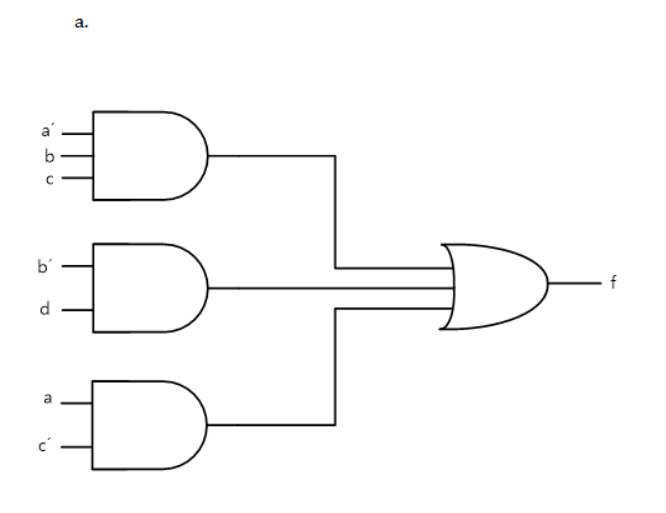
\includegraphics{res/hw01-10-a.png}

\renewcommand{\theenumi}{(\roman{enumi})}
\begin{enumerate}
\item $a'bc + b'd + ac'$
\item $a'bc + b'd + ac'$; this expression is already in \textit{sum of product} form.
\end{enumerate}

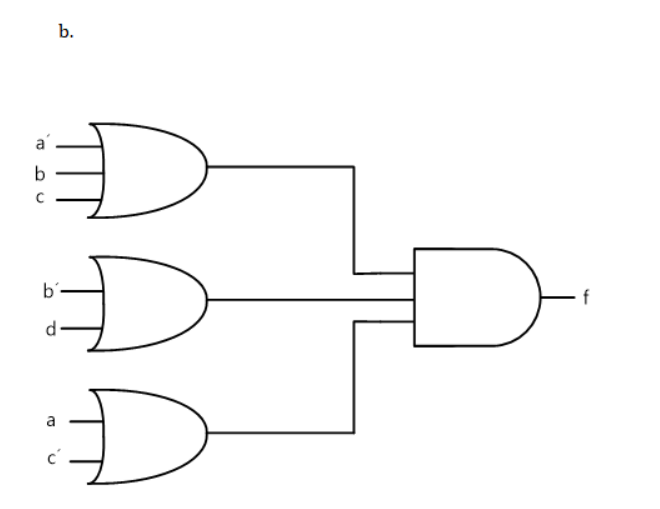
\includegraphics{res/hw01-10-b.png}
\begin{enumerate}
\item $(a' + b + c)(b' + d)(a + c')$
\item $(a' + b + c)(b' + d)(a + c')$
\begin{flalign*}
& = (a'b' + a'd + bb' + bd + b'c + cd)(a + c') & \\
& = (a'b' + a'd + bd + b'c + cd)(a + c') & \\
& = aa'b' + a'b'c' + aa'd + a'c'd + abd + bc'd + ab'c + b'cc' + acd + cc'd & \\
& = a'b'c' + a'c'd + abd + bc'd + ab'c + acd & \\
& = a'b'c' + ab'c + abd + bc'd
\end{flalign*}
\end{enumerate}

\end{document}